\documentclass[11pt]{article}
\usepackage{amssymb}
\usepackage{amsthm}
\usepackage{enumitem}
\usepackage{physics,amsmath}
\usepackage{bm}
\usepackage{adjustbox}
\usepackage{mathrsfs}
\usepackage{graphicx}
\usepackage{siunitx}
\usepackage[mathscr]{euscript}

\title{\textbf{Solved selected problems of Classical Mechanics - Gregory}}
\author{Franco Zacco}
\date{}

\addtolength{\topmargin}{-3cm}
\addtolength{\textheight}{3cm}

\newcommand{\hatr}{\bm{\hat{r}}}
\newcommand{\hatx}{\bm{\hat{x}}}
\newcommand{\haty}{\bm{\hat{y}}}
\newcommand{\hatz}{\bm{\hat{z}}}
\newcommand{\hatth}{\bm{\hat{\theta}}}
\newcommand{\hatphi}{\bm{\hat{\phi}}}
\newcommand{\hatrho}{\bm{\hat{\rho}}}
\theoremstyle{definition}
\newtheorem*{solution*}{Solution}
\renewcommand*{\proofname}{\bf{Solution}}

\begin{document}
\maketitle
\thispagestyle{empty}

\section*{Chapter 13 - The Calculus of Variations and Hamilton's Principle}

\begin{proof}{\textbf{13.1}}
    By definition, extremals are solutions of the Euler-Lagrange equation.
    In this case $F = \dot x^2/t^3$ so we have that
    \begin{align*}
        \frac{\partial F}{\partial x} = 0 \quad\quad\quad
        \frac{\partial F}{\partial \dot x} = \frac{2\dot x}{t^3} 
    \end{align*}
    Hence the Euler-Lagrange equation takes the form
    \begin{align*}
        \frac{d}{dt}\bigg(\frac{2\dot x}{t^3}\bigg) - 0 &= 0\\
        \frac{2\ddot x}{t^3} - \frac{6\dot x}{t^4} &= 0\\
        \ddot x - \frac{3\dot x}{t} &= 0
    \end{align*}
    Now we solve the equation by setting $v = \dot x$ hence
    \begin{align*}
        \frac{dv}{dt} - \frac{3v}{t} &= 0\\
        \int\frac{dv}{3v} &= \int\frac{dt}{t}\\
        \frac{\log(v)}{3} &= \log(t) + C\\
        v &= Ct^3
    \end{align*}
    by replacing again and solving the equation we have that 
    \begin{align*}
        \frac{dx}{dt} &= Ct^3\\
        \int dx &= C\int t^3dt\\
        x &= Ct^4 + D
    \end{align*}
    The admissible extremals are those that satisfy the conditions
    $x(1) = 3$ and $x(2) = 18$ this way we find the values of
    $C = 1$ and $D = 2$ so the only admissible extremal of $J[x]$ is given by
    \begin{align*}
        \hat x &= t^4 + 2
    \end{align*}

    Finally, we want to show that this extremal provides
    a global minimum of $J[x]$. Let $h$ be any admissible variation and 
    consider the variation in $J$ that it produces
    \begin{align*}
        J[\hat x + h] - J[\hat x]
        &= \int_1^2 \frac{(4t^3 + \dot h)^2}{t^3} dt
        - \int_1^2 \frac{(4t^3)^2}{t^3} dt\\
        &= \int_1^2 16t^3 + 8\dot h + \frac{\dot h^2}{t^3} dt
        - \int_1^2 16t^3 dt\\
        &= 8 \bigg[h\bigg]_{t=1}^{t=2} + \int_1^2 \frac{\dot h^2}{t^3} dt\\
        &= \int_1^2 \frac{\dot h^2}{t^3} dt
    \end{align*}
    Where we used that $h$ is an admissible extremal hence it must satisfy
    $h(1) = h(2) = 0$. Since the integral of a positive function must be
    positive we see that
    \begin{align*}
        J[\hat x + h] - J[\hat x] = \int_1^2 \frac{\dot h^2}{t^3} dt \geq 0
    \end{align*}
    Thus $\hat x$ provides the global minimum of $J[x]$.
    The global minimum value of $J$ is therefore $J [t^4 + 2] = 60$. 

\end{proof}
\cleardoublepage
\begin{proof}{\textbf{13.3}}
    We want to find the extremals of the path functional
    \begin{align*}
        L[y] = \int_0^1 \sqrt{1 + \bigg(\frac{dy}{dx}\bigg)^2} dx
    \end{align*}
    By definition, extremals are solutions of the Euler-Lagrange equation.
    In this case $F(y,\dot{y}) = \sqrt{1 + \dot{y}^2}$ so there is no explicit
    dependence on $x$ this implies that if we satisfy the equation
    \begin{align*}
        \dot{y}\frac{\partial F}{\partial\dot{y}} - F = C
    \end{align*}
    then we satisfy the Euler-Lagrange equation too, hence we have that
    \begin{align*}
        \dot{y}\frac{\dot{y}}{\sqrt{1 + \dot{y}^2}} - \sqrt{1 + \dot{y}^2} &= C\\
        \frac{\dot{y}^2 - 1 - \dot{y}^2}{\sqrt{1 + \dot{y}^2}} &= C\\
        \sqrt{1 + \dot{y}^2} &= -\frac{1}{C}\\
        \dot{y}^2 &= -1 + \frac{1}{C^2}\\
        \int y &= \frac{\sqrt{1-C^2}}{C^2} \int dx\\
        y &= \frac{\sqrt{1-C^2}}{C^2} x + D
    \end{align*}
    Where $D$ is a constant of integration. Now applying the given
    initial and end conditions we get that $C = 1$ and $D = 0$ so 
    the admissible extremal is
    \begin{align*}
        \hat y &= 0        
    \end{align*}
    But this is a constant solution so it may or may not be a solution to the
    Euler-Lagrange equation, we must check, hence we have that
    \begin{align*}
        \frac{d}{dt}\bigg(\frac{\partial F}{\partial \dot y}\bigg) - \frac{\partial F}{\partial y} = 0\\
        \frac{d}{dt}\bigg(\frac{\dot{y}}{\sqrt{1 + \dot{y}^2}}\bigg) - 0 = 0\\
        \frac{\ddot{y}}{(1 + \dot{y}^2)^{3/2}} = 0
    \end{align*}
    So $\hat y = 0$ is a solution to the Euler-Lagrange equation and therefore
    an extremal.
\cleardoublepage
    Finally, we want to check $\hat y$ provides a global minimum for $L$.
    Let $h$ be any admissible variation and consider the variation in $L$
    that it produces
    \begin{align*}
        L[\hat y + h]
        % - L[\hat y]
        &= \int_0^1 \sqrt{1 + (\dot{\hat y} + \dot h)^2} dx\\
        % - \int_0^1 \sqrt{1 + \dot{\hat y}^2} dx\\
        &= \int_0^1 \sqrt{1 + \dot h^2} dx
        % - \int_0^1 dx\\
        % &= \int_0^1 \sqrt{1 + \dot h^2} dx - 1\\
    \end{align*}
    Also, we know that
    $$\int_0^1 \sqrt{1 + \dot{\hat y}^2} dx = \int_0^1 dx = 1$$
    And we have that
    \begin{align*}
        \int_0^1 \sqrt{1 + \dot h^2} dx \geq 1 = \int_0^1 dx
    \end{align*}
    Therefore $\hat y$ provides a local minimum for $L$.
\end{proof}
\cleardoublepage
\begin{proof}{\textbf{13.5}}
    Let us analyze the following system
    \begin{center}
        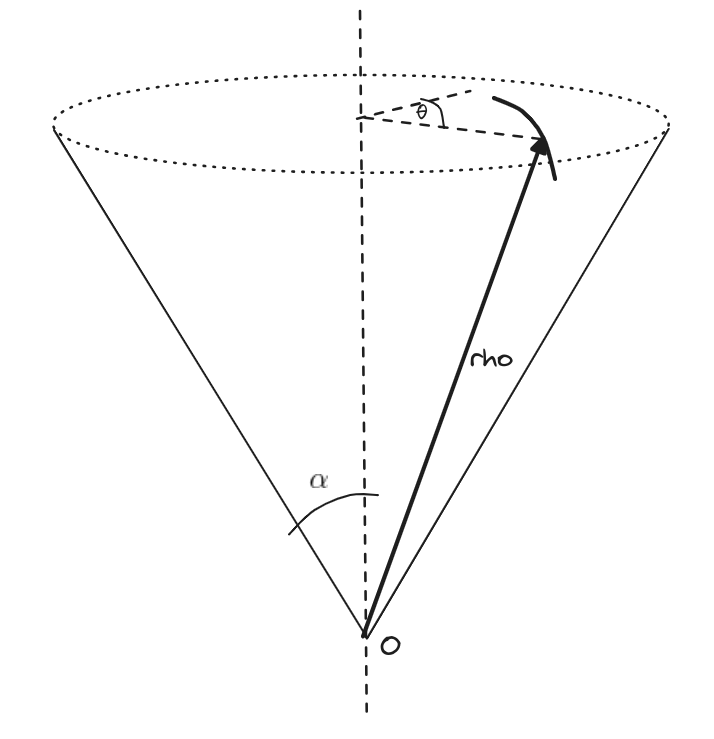
\includegraphics[scale=0.4]{ch13-5.png}
    \end{center}
    From this, we can write the differential length as
    \begin{align*}
        (ds)^2 = (d\rho)^2 + (\rho \sin\alpha d\theta)^2
    \end{align*}
    So integrating we get the length functional as follows
    \begin{align*}
        L = \int_{-\pi/2}^{\pi/2} ds =
        \int_{-\pi/2}^{\pi/2} \sqrt{\left(\frac{d\rho}{d\theta}\right)^2 + (\rho \sin\alpha)^2}~d\theta
    \end{align*}
    In this case, we have that
    $F(\rho,\dot{\rho}) = \sqrt{\dot\rho^2 + (\rho\sin\alpha)^2}$
    so there is no explicit dependence on $\theta$ this implies that if we
    satisfy the equation
    \begin{align*}
        \dot{\rho}\frac{\partial F}{\partial\dot{\rho}} - F = C
    \end{align*}
    then we satisfy the Euler-Lagrange equation too, hence we have that
    \begin{align*}
        \dot{\rho}\frac{\dot{\rho}}{\sqrt{\dot\rho^2 + (\rho\sin\alpha)^2}}
        - \sqrt{\dot\rho^2 + (\rho\sin\alpha)^2} &= C\\
        \frac{\dot{\rho}^2 - \dot\rho^2 - (\rho\sin\alpha)^2}
        {\sqrt{\dot\rho^2 + (\rho\sin\alpha)^2}} &= C\\
        \sqrt{\dot\rho^2 + (\rho\sin\alpha)^2} &= -\frac{(\rho\sin\alpha)^2}{C}\\
        \dot\rho^2  &= - (\rho\sin\alpha)^2 + \frac{(\rho\sin\alpha)^4}{C^2}\\
        \frac{d\rho}{d\theta} &= (\rho\sin\alpha)\sqrt{\frac{(\rho\sin\alpha)^2}{C^2} - 1}\\
    \end{align*}
    Now  we can integrate the equation as follows
    \begin{align*}
        \int \frac{d\rho}{(\rho\sin\alpha)\sqrt{\frac{(\rho\sin\alpha)^2}{C^2} - 1}}
        &= \int d\theta\\
        \frac{\arctan(\sqrt{\frac{(\rho\sin\alpha)^2}{C^2} - 1})}{\sin\alpha}
        &= \theta + D\\
        \arctan(\sqrt{\frac{(\rho\sin\alpha)^2}{C^2} - 1})
        &= (\theta + D)\sin\alpha\\
        \frac{(\rho\sin\alpha)^2}{C^2} - 1
        &= \tan^2\left((\theta + D)\sin\alpha\right)\\
        \rho &= \frac{C}{\sin\alpha}
        \sqrt{\tan^2\left((\theta + D)\sin\alpha\right) + 1}\\
        \rho &= \frac{C}{\sin\alpha}\sec((\theta + D)\sin\alpha)
    \end{align*}
    This is the equation for the extremals of $L$.
    Now applying the given initial and end conditions we get that
    \begin{align*}
        a = \frac{C}{\sin\alpha}\sec(-(\pi/2 - D)\sin\alpha)
        &= \frac{C}{\sin\alpha}\sec((\pi/2 + D)\sin\alpha)
    \end{align*}
    which implies that $D = 0$ and $C$ is
    \begin{align*}
        C \sec\left(\frac{\pi\sin\alpha}{2}\right) &= a\sin\alpha\\
        C &= \frac{a\sin\alpha}{\sec\left(\frac{\pi\sin\alpha}{2}\right)}
    \end{align*}
    Replacing the values for $C$ and $D$ we get that the admissible extremal is
    \begin{align*}
        \rho &=
        \frac{a\sec(\theta\sin\alpha)}{\sec(\frac{\pi\sin\alpha}{2})}\\
        \rho &=
        \frac{a\cos(\frac{\pi\sin\alpha}{2})}{\cos(\theta\sin\alpha)}\\
    \end{align*}
    \cleardoublepage
    Finally, we want to verify that this extremal is the same as the shortest
    path that would be obtained by developing the cone onto a plane.
    If we develop the cone onto a plane, we get that the path is a vertical
    line in the plane as shown below
    \begin{center}
        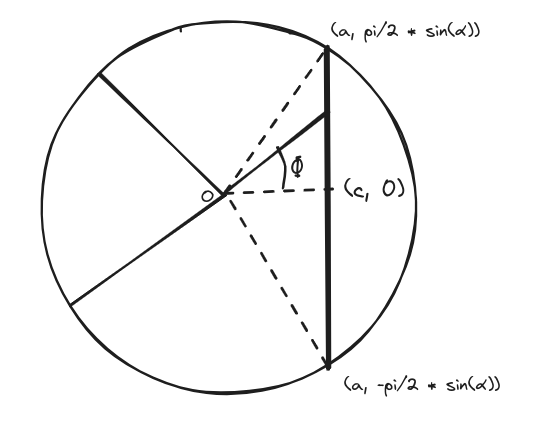
\includegraphics[scale=0.4]{ch13-5_1.png}
    \end{center}
    where the angle in the plane is given by $\phi = \theta \sin\alpha$.
    We know that the equation of a straight vertical line in polar coordinates
    is given by
    \begin{align*}
        \rho\cos(\phi) &= c
    \end{align*}
    where $c$ is the value of $\rho$ when $\phi = 0$ and from the drawing
    above we have that $\cos(\pi/2\sin(\alpha)) = c/a$ hence 
    \begin{align*}
        \rho\cos(\theta\sin\alpha) &= a\cos(\frac{\pi\sin(\alpha)}{2})
    \end{align*}
    Which is the admissible extremal that we have such that it satisfies
    the Euler-Lagrange equation.
\end{proof}
\cleardoublepage
\begin{proof}{\textbf{13.7}}
    We want to find the extremals of
    \begin{align*}
        J[y] = \int_{-a}^a y\sqrt{1 + \dot y^2}~dx
    \end{align*}
    In this case, we have that
    $F(y,\dot{y}) = y \sqrt{1 + \dot y^2}$
    so there is no explicit dependence on $x$ this implies that if we
    satisfy the equation
    \begin{align*}
        \dot{y}\frac{\partial F}{\partial\dot{y}} - F = C
    \end{align*}
    then we satisfy the Euler-Lagrange equation too, hence we have that
    \begin{align*}
        \dot{y} \frac{y\dot y}{\sqrt{1 + \dot y^2}} - y \sqrt{1 + \dot y^2} &= C\\
        \frac{\dot yy^2 - (y(1  + \dot{y}^2))}{\sqrt{1 + \dot y^2}} &= C\\
        \frac{y}{\sqrt{1 + \dot y^2}} &= -C\\
        y^2 &= C^2(1 + \dot y^2)\\
        \sqrt{\frac{y^2}{C^2} - 1} &=  \dot y
    \end{align*}
    Now we can solve this equation by separation as follows
    \begin{align*}
        \int \frac{dy}{\sqrt{\frac{y^2}{C^2} - 1}} &= \int dx\\
        C\int \frac{dy}{\sqrt{y^2 - C^2}} &= \int dx\\
        \cosh^{-1}\left(\frac{y}{C}\right) &= \frac{x}{C} + D\\
        y &= C\cosh\left(\frac{x}{C} + D\right)
    \end{align*}
    Which is the form of the extremals of $J[y]$ we wanted.

    To determine the values of $C$ and $D$ we use the initial and end
    conditions. We know that $y(-a) = y(a) = b$ hence we have that
    \begin{align*}
        C\cosh\left(\frac{a}{C} + D\right) &= C\cosh\left(-\frac{a}{C} + D\right)\\
        \cosh\left(\frac{a}{C} + D\right) &= \cosh\left(\frac{a}{C} - D\right)\\
        \frac{a}{C} + D &= \frac{a}{C} - D\\
        D &= 0
    \end{align*}
    So the initial and end conditions are satisfied only if $D = 0$.

    Naming $\lambda = a/C$ we see that
    \begin{align*}
        \cosh\left(\frac{a}{C}\right) &= \frac{b}{C}\\
        \cosh(\lambda) &= \frac{b}{a} \lambda
    \end{align*}
    We see that depending the value of $b/a$ the curve $\cosh(\lambda)$ will or
    will not intersect the line $(b/a) \lambda$ for example if we take
    $b/a = 1$ and we plot both curves we have that
    \begin{center}
        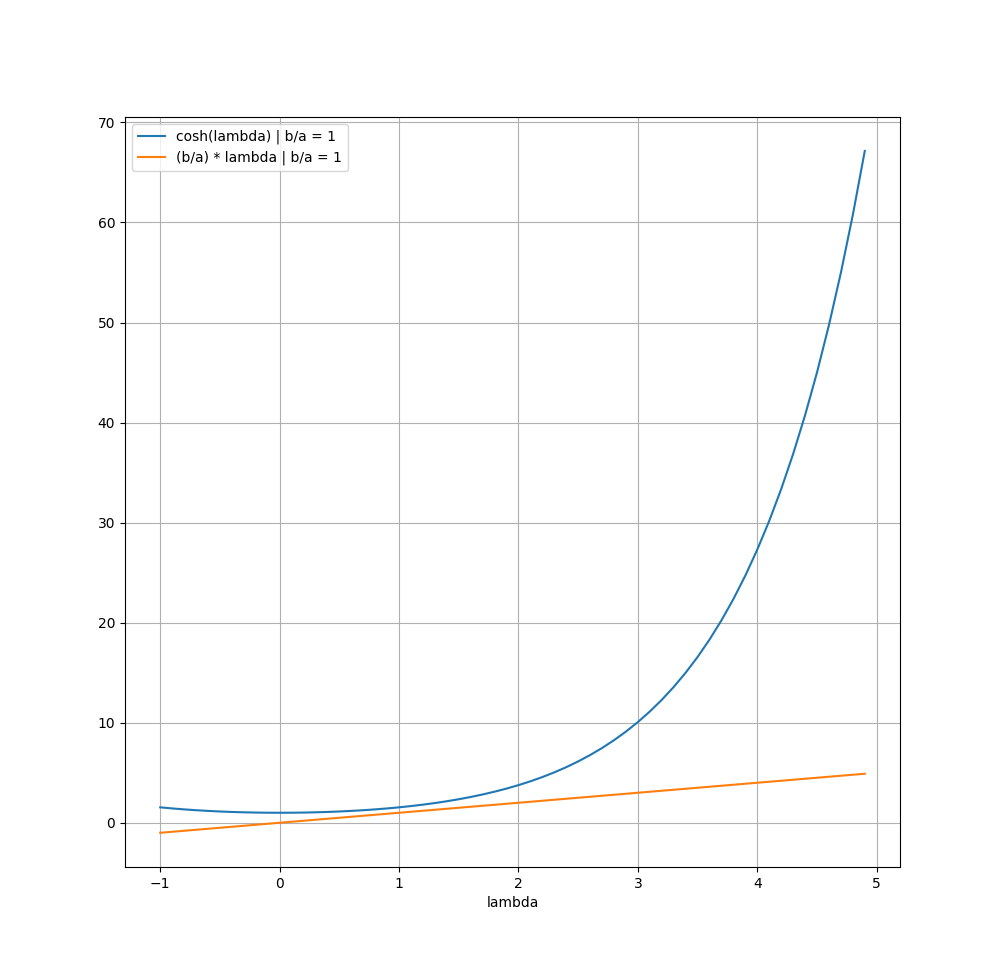
\includegraphics[scale=0.4]{ch13-7_1.png}
    \end{center}
    Where we see that the curves don't intersect hence there is no solution
    to the equation so no value of $C$ satisfies the initial and
    end conditions and therefore there are no admissible extremals
    for this case.
    If we set $b/a = 1.51$ we see that the curves do intersect and this value
    seems to be quite close to the critical point as shown below.
    \begin{center}
        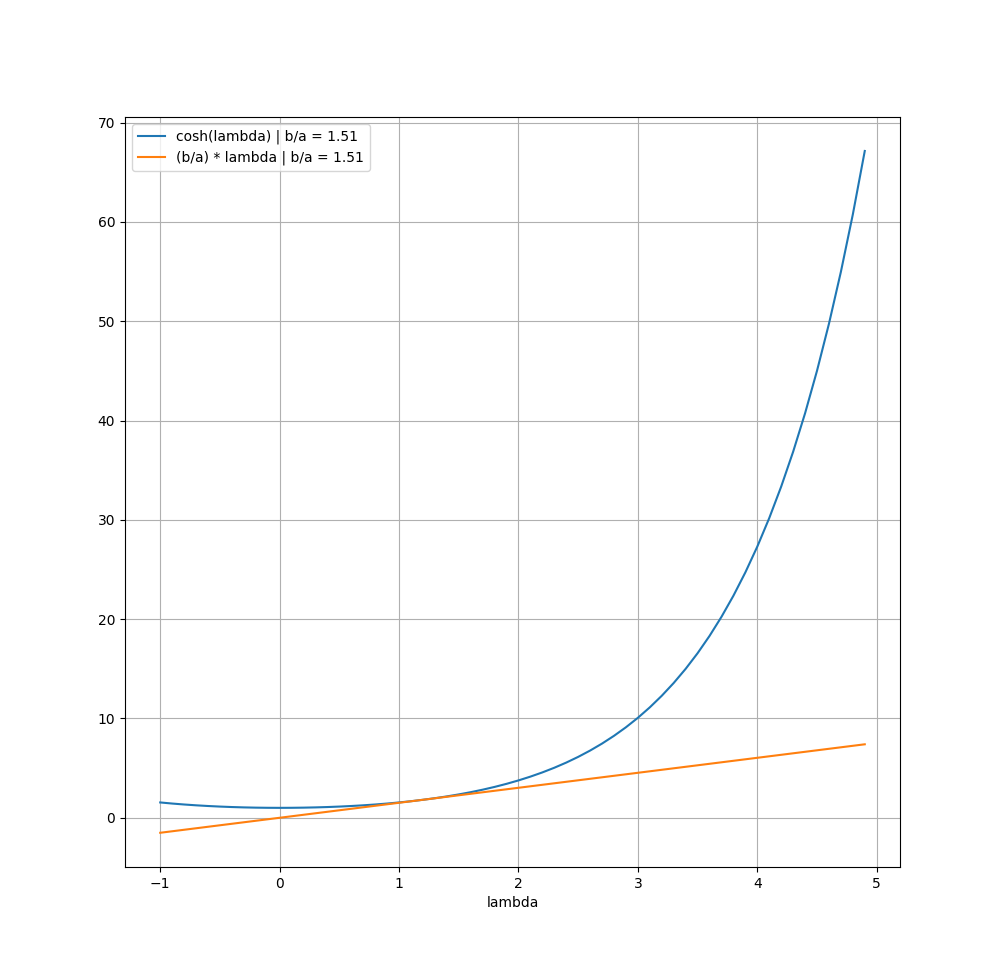
\includegraphics[scale=0.4]{ch13-7_2.png}
    \end{center}
    
    If we choose $b/a = 2$ the curves intersect at two points
    $\lambda_1 = 0.5893$ and $\lambda_2 = 2.1268$ as shown below
    \begin{center}
        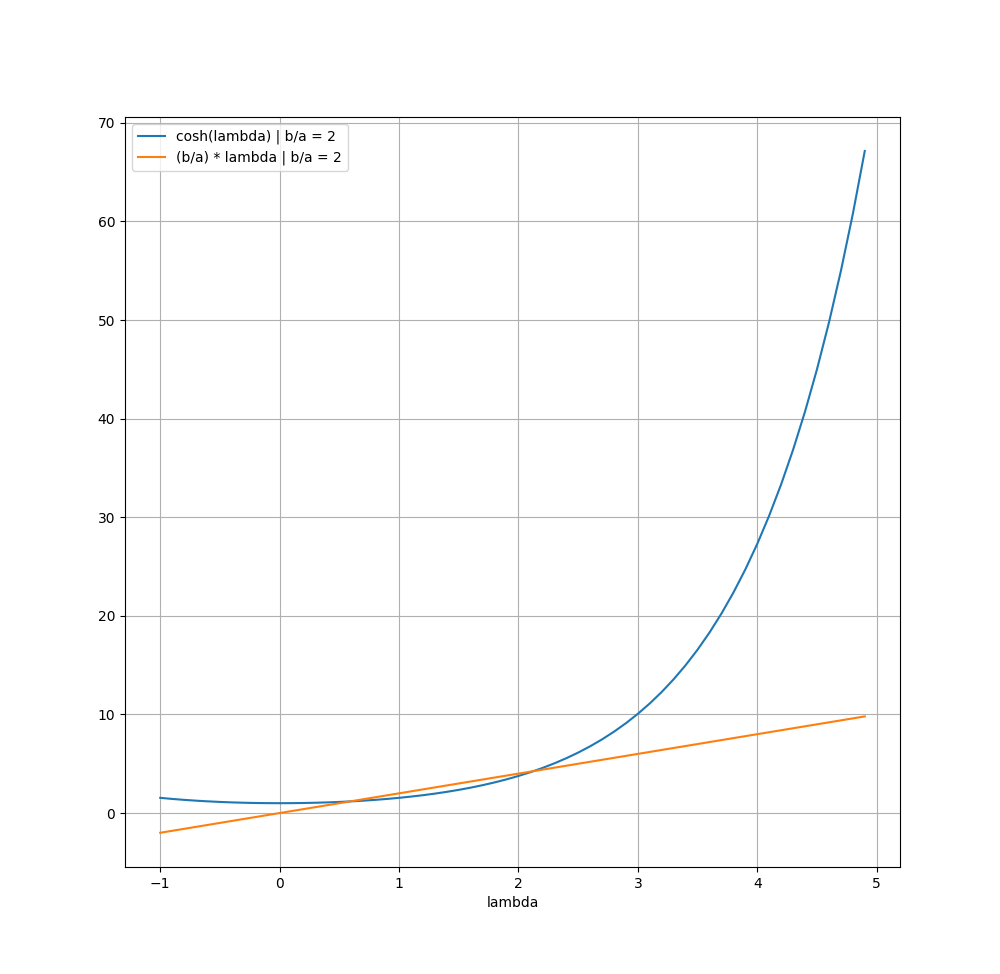
\includegraphics[scale=0.4]{ch13-7_3.png}
    \end{center}
    
    \cleardoublepage
    Now taking $a = 1$ we plot both extremals where we use
    $C_1 = 1/\lambda_1$ and $C_2 = 1/\lambda_2$
    \begin{center}
        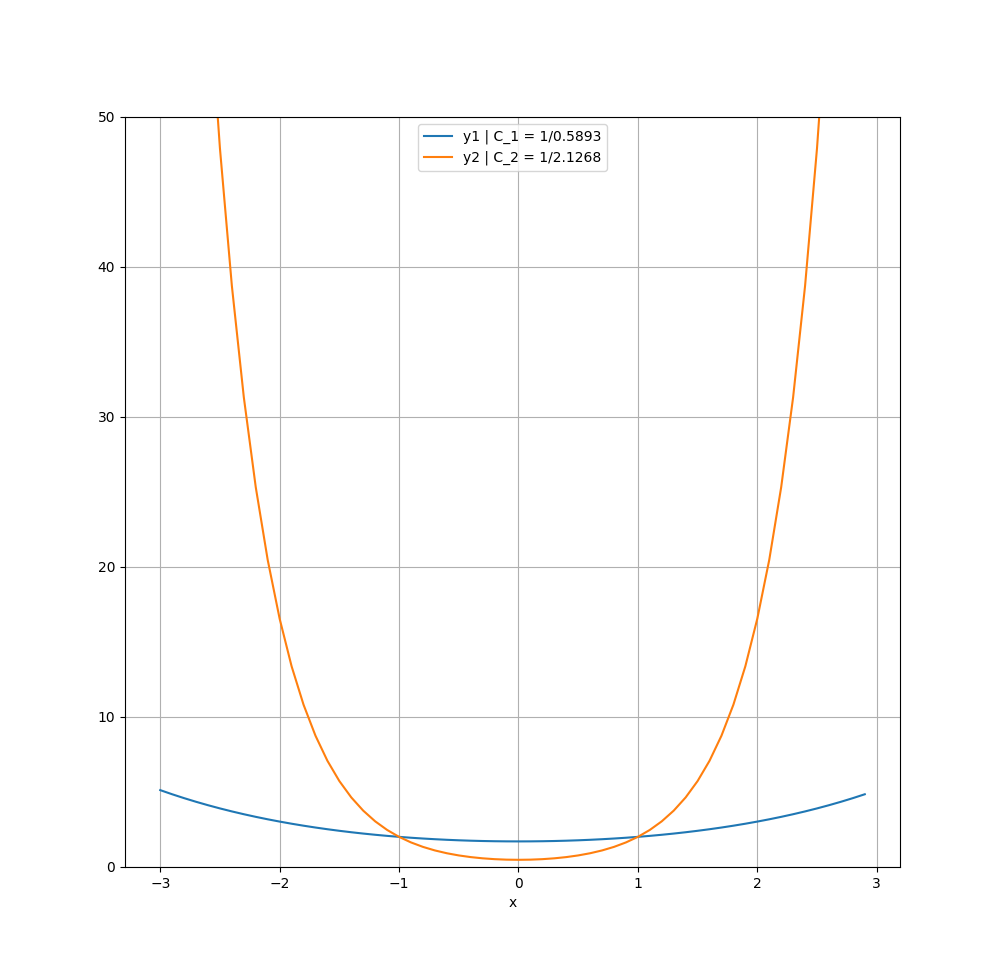
\includegraphics[scale=0.4]{ch13-7_4.png}
    \end{center}
    By the shape of the curve, we can guess that the blue curve represents the
    soap film.
\end{proof}
\cleardoublepage
\begin{proof}{\textbf{13.9}}
    We want to determine Feremat's time functional, for this, we need 
    first, the line element in cylindrical polar coordinates i.e.
    \begin{align*}
        ds^2 &= dr^2 + r^2d\theta^2
    \end{align*}
    So Fermat's time functional is given by
    \begin{align*}
       T[r] &= c^{-1}\int n ds\\
        &= c^{-1}\int n \sqrt{dr^2 + r^2d\theta^2}\\
        &= c^{-1}\int_{\theta_0}^{\theta_1} n
        \sqrt{\left(\frac{dr}{d\theta}\right)^2 + r^2}~d\theta
    \end{align*}
    Which is the expression we wanted. Using the calculus of variations 
    we note that $F(r, \dot r) = n\sqrt{\dot r^2 + r^2}$ which does not
    depends on $\theta$ so if we satisfy the equation
    \begin{align*}
        \dot{r}\frac{\partial F}{\partial\dot{r}} - F = C
    \end{align*}
    then we satisfy the Euler-Lagrange equation too, hence we have that
    \begin{align*}
        \dot{r}~\frac{n\dot{r}}{\sqrt{\dot r^2 + r^2}} - n \sqrt{\dot r^2 + r^2} &= C\\
        n\left(\frac{\dot{r}^2}{\sqrt{\dot r^2 + r^2}} - \sqrt{\dot r^2 + r^2}\right) &= C\\
        n\left(\frac{\dot{r}^2 - (\dot{r}^2 + r^2)}{\sqrt{\dot r^2 + r^2}}\right) &= C\\
        \frac{nr^2}{\sqrt{\dot r^2 + r^2}} &= C
    \end{align*}
    Let now $\dot{r} = r \tan \psi$ then we get that
    \begin{align*}
        \frac{nr^2}{\sqrt{(r \tan \psi)^2 + r^2}} &= C\\
        \frac{nr}{\sqrt{\tan^2\psi + 1}} &= C\\
        \frac{nr}{\frac{1}{\cos\psi}\sqrt{\sin^2\psi + \cos^2\psi}} &= C\\
        nr\cos\psi &= C
    \end{align*}
    Which is Snell's law for this case as we wanted.
    Finally, if we consider a circular ray with center at the origin then must
    be that $\psi = 0$ hence we get that $nr = a$ where we named the constant
    as $a$ then $n = a/r$.
\end{proof}
\cleardoublepage
\begin{proof}{\textbf{13.10}}
    Let a particle of mass $2~kg$ move under uniform gravity where
    $g = 10~m/s^2$ along the z-axis, which points vertically downwards.
    The lagrangian in this case is given by
    \begin{align*}
        L(z, \dot{z}) &= T(\dot{z}) - V(z)\\
            &= \frac{1}{2}m\dot{z}^2 - (- mgz)\\
            &= \dot{z}^2 + 20z
    \end{align*}
    Then the action functional for a time interval $[0,2]$ is given by
    \begin{align*}
        S[z] &= \int_0^2 L(z, \dot{z})~dt
            = \int_0^2 (\dot{z}^2 + 20z) dt
    \end{align*}
    Because of Hamilton's principle, $z(t) = 5t^2$ makes stationary the
    action functional. Let us compute the value of $S[z]$
    \begin{align*}
        S[z] &= \int_0^2 100t^2 + 100t^2~dt\\
            &= \left[\frac{200t^3}{3}\right]_{t=0}^{t=2}\\
            &= \frac{1600}{3}
    \end{align*}
    Now let us consider an admissible variation of $z(t)$ as follows
    \begin{align*}
        S[z + h] &= \int_0^2 ((10t + \dot h)^2 + 20(5t^2 + h))~dt\\
            &= \int_0^2 200t^2 + 20t\dot h + \dot h^2 + 20h~dt\\
            &= \left[\frac{200t^3}{3}\right]_{t=0}^{t=2}
            + [20th]_{t=0}^{t=2} + \int_0^2 \dot h^2~dt\\
            &= \frac{1600}{3} + 0 + \int_0^2 \dot h^2~dt
    \end{align*}
    We used that $h$ is an admissible variation and hence $h(0)=h(2)=0$.
    So we see that $S[z + h] = S[z] + \int_0^2 \dot h^2~dt$ and since 
    the integral of a positive function $\dot h^2$ must be positive then
    $$S[z + h] = S[z] + \int_0^2 \dot h^2~dt \geq S[z]$$
    so $z(t) = 5t^2$ provides a global minimum for $S[z]$.
\end{proof}
\cleardoublepage
\begin{proof}{\textbf{13.11}}
    In this case, we are given the Lagrangian of the system which is
    \begin{align*}
        L &= \dot{q}^2 - 4q^2
    \end{align*}
    So the Lagrange equation in this case is
    \begin{align*}
        \frac{d}{dt}\left(\frac{\partial L}{\partial \dot q}\right)
        - \frac{\partial L}{\partial q} &= 0\\
        \ddot{q} + 4q &= 0
    \end{align*}
    We want to verify that $q^* = \sin 2t$ is a motion of the oscillator then
    it must be a solution to the Lagrange equation we got, we check this below
    \begin{align*}
        \frac{d^2\sin(2t)}{dt^2} + 4\sin(2t) = -4\sin(2t) + 4\sin (2t) &= 0
    \end{align*}
    So we see $q^*$ is a solution to the Lagrange equation and therefore
    a motion of the oscillator.

    The action functional is given by
    \begin{align*}
        S[q] &= \int_0^\tau \dot{q}^2 - 4q^2~dt
    \end{align*}
    and since $q^*$ is a solution to the Lagrange equation it must make $S$
    stationary, we check this below. Let $h(t)$ be an admissible variation then 
    \begin{align*}
        S[q^* + h] - S[q^*] 
        &= \int_0^\tau (2\cos 2t + \dot h)^2 - 4(\sin 2t + h)^2~dt\\
        &\quad\quad- \int_0^\tau (2\cos 2t)^2 - 4(\sin 2t)^2~dt\\
        &= 4\int_0^\tau \cos^2 2t + \dot h\cos 2t + \frac{\dot h^2}{4}
        - \sin^2 2t  - 2h\sin 2t - h^2~dt\\
        &\quad\quad- 4\int_0^\tau \cos^2 2t - \sin^2 2t~dt\\
        &= 4\int_0^\tau \cos 4t + \dot h\cos 2t + \frac{\dot h^2}{4}
        - 2h\sin 2t - h^2~dt\\
        &\quad\quad- 4\int_0^\tau \cos 4t~dt\\
        &= 4\bigg[h\cos 2t\bigg]_{0}^\tau
        + 4\int_0^\tau \left(\frac{\dot h^2}{4} - h^2 \right)~dt\\
        &= \int_0^\tau \left(\dot h^2 - 4h^2 \right)~dt
    \end{align*}
    We used that $h(\tau) = h(0) = 0$. It follows that
    \begin{align*}
        \left|S[q^* + h] - S[q^*]\right|
        &= \left|\int_0^\tau \left(\dot h^2 - 4h^2 \right)~dt\right|\\
        &\leq  \int_0^\tau \left|\dot h^2 - 4h^2 \right|~dt\\
        &\leq  \int_0^\tau |\dot h|^2 + |4h|^2~dt\\
        &\leq  \int_0^\tau (\max|\dot h|)^2 + (\max|4h|)^2~dt\\
        &= \tau((\max|\dot h|)^2 + (\max|4h|)^2)\\
        &\leq \tau(\max|\dot h| + 4\max|h|)^2 = \tau\|h\|^2
    \end{align*}
    Hence $\left|S[q^* + h] - S[q^*]\right| = O(\|h\|^2)$ which by definition,
    means that $q^*$ makes the action functional $S[q]$ stationary.

    Let us take now a time interval $0 \leq t \leq \pi$ then
    \begin{align*}
        S[q^*] = 4 \int_0^\pi \cos(4t) = 0
    \end{align*}
    If $h = \epsilon \sin(4t)$ we have that
    \begin{align*}
        S[q^* + h] - S[q^*] 
        &= \int_0^\pi \left((4\epsilon\cos 4t)^2 - 4(\epsilon\sin 4t)^2 \right)~dt\\
        &= 4\epsilon^2\int_0^\pi 4\cos^2 4t - \sin^2 4t~dt\\
        &= \epsilon^2\left[\frac{5}{4}\sin(8t) + 6t\right]_{t=0}^{t=\pi}\\
        &= \epsilon^2[6\pi - 0] = \epsilon^26\pi
    \end{align*}
    So we see that $S[q^* + h] = S[q^*] + \epsilon^26\pi \geq S[q^*] = 0$.

    On the other hand, if $h = \epsilon \sin(t)$ in the same way we have that
    \begin{align*}
        S[q^* + h] - S[q^*] 
        &= \int_0^\pi \left((\epsilon\cos t)^2 - 4(\epsilon\sin t)^2 \right)~dt\\
        &= \epsilon^2\int_0^\pi \cos^2 t - 4\sin^2 t~dt\\
        &= \epsilon^2\left[\frac{1}{2}(5\sin(t)\cos(t) - 3t)\right]_{t=0}^{t=\pi}\\
        &= \epsilon^2\left[-\frac{3\pi}{2} - 0\right] = -\epsilon^2\frac{3\pi}{2}
    \end{align*}
    So we see that $S[q^* + h] = S[q^*] -\epsilon^2\frac{3\pi}{2} \leq S[q^*] = 0$.
    
    Therefore we have that $q^*$ does not make $S$ a minimum or a maximum.
\end{proof}
\cleardoublepage
\begin{proof}{\textbf{13.12}}
    Given that the particle is constrained to move over a smooth fixed surface
    under no forces other than the force of constraint, and the former do no work
    the lagrangian for the system is $L = \frac{1}{2}m\bm{\dot{r}}^2$.
    We want to check if the path of a particle must be a geodesic i.e.
    makes the Lenght functional
    \begin{align*}
        L[\bm{r}] &= \int_{t_0}^{t_1} |\bm{\dot{r}}| dt
    \end{align*}
    stationary. We know from the conservation of energy that
    $T = \text{constant}$ which implies that a particle that moves along the
    surface must have a constant velocity
    so
    $$L[\bm{r}] = |\bm{\dot{r}}| \Delta t $$
    
    On the other hand, we know from Hamilton's principle that a
    motion of a particle on the surface must satisfy the Lagrange equations
    and hence it must make the action functional stationary.

    So let $\bm{r}^*$ be the actual path of a particle and $h$ be
    an admissible variation such that $\bm{r} = \bm{r}^* + h$, we know that
    \begin{align*}
        S[\bm{r}^* + h] - S[\bm{r}^*] = O(h^2)
    \end{align*}
    hence
    \begin{align*}
        \frac{1}{2}m\int_{t_0}^{t_1} \bm{\dot{r}}^2 dt &= 
        \frac{1}{2}m\int_{t_0}^{t_1} \bm{\dot{r}}^{*2} dt + 
        O(h^2)\\
        &= \frac{1}{2}m |\bm{\dot{r}}^*|^2\Delta t +  O(h^2)
    \end{align*}
    Where we used that $\bm{\dot{r}^*}$ is constant since $\bm{r^*}$ is the
    actual path of a particle.
    Given the above equation
    must be true for any path we can traverse $\bm{r} = \bm{r^*} + h$
    with constant velocity i.e. we can take out of the integral $\bm{\dot{r}}^2$
    then we have that
    \begin{align*}
        \frac{1}{2}m |\bm{\dot{r}}|^2\Delta t
        &= \frac{1}{2}m |\bm{\dot{r}}^*|^2\Delta t +  O(h^2) 
    \end{align*}
    Finally, by replacing $L[\bm{r}]$ we get that
    \begin{align*}
        \frac{1}{2}m \frac{L[\bm{r}]^2}{\Delta t}
        &= \frac{1}{2}m \frac{L[\bm{r^*}]^2}{\Delta t} +  O(h^2) 
    \end{align*}

    Which implies that $L[\bm{r}] = L[\bm{r}^*] + O(h^2)$.
    Therefore the Length functional is stationary too.
\end{proof}
\cleardoublepage
\begin{proof}{\textbf{13.13}}
    Let $L(\bm{q}, \bm{\dot{q}}, t)$ be the Lagrangian of the system then the
    motion of the system $\bm{q}^*$ will satisfy the Lagrange equation 
    \begin{align*}
        \frac{d}{dt}\bigg(\frac{\partial L}{\partial \bm{\dot{q}}}\bigg)
        - \frac{\partial L}{\partial \bm{q}} = 0
    \end{align*}
    but also $\bm{q}^*$ makes the action functional stationary.
    We want to check that a modification to the Lagrangian of the system to
    $L' = L + \frac{d}{dt}g(\bm{q},t)$ still preserves $\bm{q}^*$ as a motion
    of the system hence it must make the action functional with the
    new Lagrangian stationary.
    
    Let us compute the action functional for this case
    \begin{align*}
        S'[\bm{q}] &= \int_{t_0}^{t_1} L'(\bm{q}, \bm{\dot{q}}, t)~dt\\
        S'[\bm{q}] &= \int_{t_0}^{t_1} L + \frac{d}{dt}g(\bm{q},t)~dt\\
        S'[\bm{q}] &= S[\bm{q}] + \int_{t_0}^{t_1} dg(\bm{q},t)\\
        S'[\bm{q}] &= S[\bm{q}] + \bigg[g(\bm{q},t)\bigg]_{t_0}^{t_1}\\
        S'[\bm{q}] &= S[\bm{q}] + [g(\bm{q},t_1) - g(\bm{q},t_0)]
    \end{align*}
    So we see that $S'[\bm{q}]$ differs from $S[\bm{q}]$ only on a constant
    value, so $S'[\bm{q}]$ will be still stationary for $\bm{q}^*$.
    Therefore if $\bm{q}^*$ is a motion of the system it still will be if
    we change the Lagrangian to $L'$.    
\end{proof}
\cleardoublepage
\begin{proof}{\textbf{13.14}}
    Let  $\mathcal{C}$ be a path lying on the surface that connects $P$ and $Q$.
    We want to determine the length of $\mathcal{C}$. We know that the line
    element in cylindrical coordinates is 
    \begin{align*}
        ds^2 &= dr^2 + r^2d\theta^2 + dz^2
    \end{align*}
    Given that $P$ and $Q$ are separated by $\pi$ radians in cylindrical
    coordinates we integrate the length functional between
    $-\pi/2$ and $\pi/2$ as follows
    \begin{align*}
       L[r] &= \int_{-\pi/2}^{\pi/2} ds\\
        &= \int_{-\pi/2}^{\pi/2} \sqrt{dr^2 + r^2d\theta^2 + dz^2}\\
        &= \int_{-\pi/2}^{\pi/2}
        \sqrt{\left(\frac{dr}{d\theta}\right)^2 + r^2 + \left(\frac{dz}{d\theta}\right)^2}~d\theta
    \end{align*}
    Also, we know that the surface of the paraboloid is given by $z = x^2 + y^2$
    so in cylindrical coordinates, we have that
    $z = (r\cos\theta)^2 + (r\sin\theta)^2 = r^2$
    which implies that $dz/d\theta = 2r\dot{r}$ where $\dot r = dr/d\theta$ hence
    \begin{align*}
        L[r] &= \int_{-\pi/2}^{\pi/2}
        \sqrt{\dot{r}^2
        + r^2
        + \left(2r\dot{r}\right)^2}~d\theta\\
        &= \int_{-\pi/2}^{\pi/2}
        \sqrt{r^2 + (1 + 4r^2)\dot{r}^2}~d\theta
    \end{align*}
    We see that $F(r, \dot{r}) = \sqrt{r^2 + (1 + 4r^2)\dot{r}^2}$ so
    the Euler-Lagrange equation is given by
    \begin{align*}
        \frac{d}{d\theta}\left(\frac{\partial F}{\partial \dot r}\right)
        - \frac{\partial F}{\partial r} &= 0\\
        \frac{d}{d\theta}\bigg(\frac{(4r^2+1)\dot{r}}{\sqrt{r^2 + (1 + 4r^2)\dot{r}^2}}\bigg)
        - \frac{(4\dot r^2+1)r}{\sqrt{r^2 + (1 + 4r^2)\dot{r}^2}} &= 0\\
    \end{align*}
    And we see that 
    \begin{align*}
        \frac{d}{d\theta}\bigg(\frac{(4r^2+1)\dot{r}}{\sqrt{r^2 + (1 + 4r^2)\dot{r}^2}}\bigg)
        &= \frac{2r(4r^2(4\dot r + 1) + 4\dot r - 1)\dot r^2 + (4r^2 + 1)(r^2(4\dot r + 2) + \dot r)\ddot r}
        {2(r^2 + (1 + 4r^2)\dot r^2)^{3/2}}\\
        &= \frac{4r(4r^2 + 1)\dot r^4 + r(4r^2 - 1)\dot r^2 + r^2(4r^2 + 1)\ddot r}
        {(r^2 + (1 + 4r^2)\dot r^2)^{3/2}}\\
    \end{align*}
    So the Euler-Lagrange equation is
    \begin{align*}
        \frac{(4\dot r^2+1)r}{\sqrt{r^2 + (1 + 4r^2)\dot{r}^2}}
        &= \frac{4r(4r^2 + 1)\dot r^4 + r(4r^2 - 1)\dot r^2 + r^2(4r^2 + 1)\ddot r}
        {(r^2 + (1 + 4r^2)\dot r^2)^{3/2}}\\
        (4r\dot r^2+r)(r^2 + (1 + 4r^2)\dot r^2)
        &= 4r(4r^2 + 1)\dot r^4 + r(4r^2 - 1)\dot r^2 + r^2(4r^2 + 1)\ddot r\\
        r(4r^2 + 1)\ddot r  &= (4\dot r^2 + 1)(r^2 + (1 + 4r^2)\dot r^2)
        - 4(4r^2 + 1)\dot r^4 - (4r^2 - 1)\dot r^2
    \end{align*}
    So finally we get that
    \begin{align*}
        \ddot r  &= \frac{(4\dot r^2 + 1)(r^2 + (1 + 4r^2)\dot r^2)
        - 4(4r^2 + 1)\dot r^4 - (4r^2 - 1)\dot r^2}{r(4r^2 + 1)}
    \end{align*}
    Now naming $\dot r = u$ we have that
    \begin{align*}
        \dot u  &= \frac{(4u^2 + 1)(r^2 + (1 + 4r^2)u^2)
        - 4(4r^2 + 1)u^4 - (4r^2 - 1)u^2}{r(4r^2 + 1)}
    \end{align*}
    Hence we have a system of differential equations that we can solve
    numerically assuming that $r(0) = \lambda$ and $u(0) = \dot{r}(0) = 0$
    in this way, we get that
    \begin{center}
        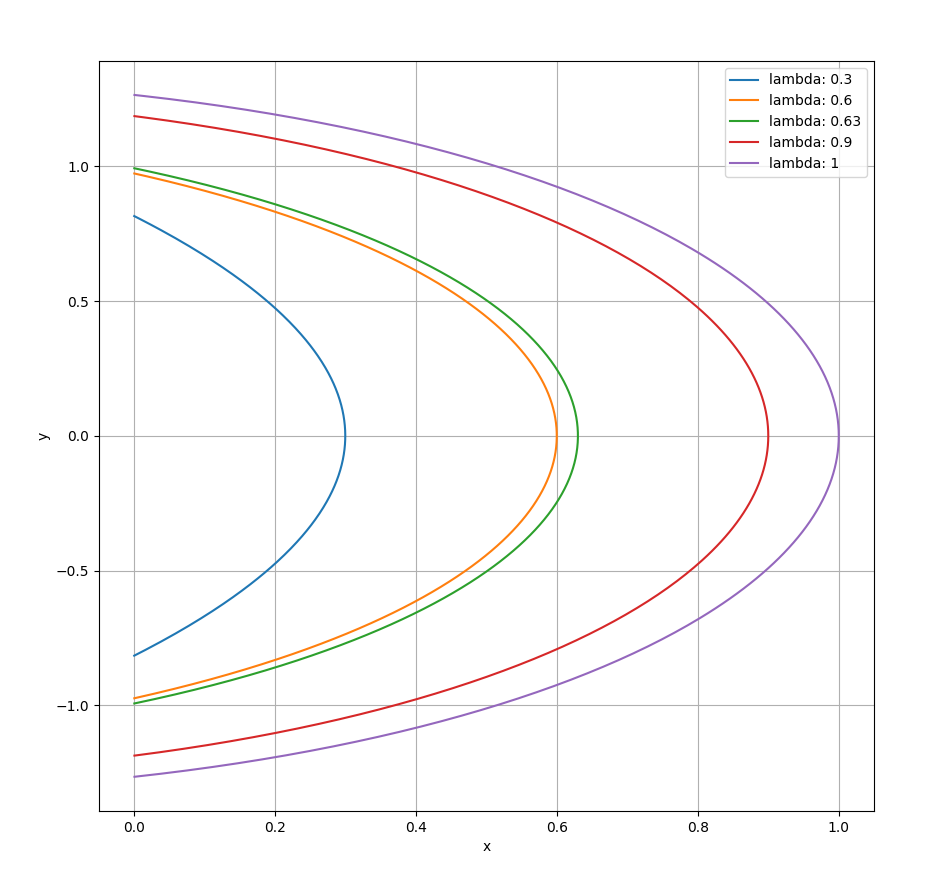
\includegraphics[scale=0.5]{ch13-14_2.png}
    \end{center}
    Which is the projection of the curve over the $z=0$ plane. Observing this
    plot we see that the right value for $\lambda$ is around 0.63.
    Finally, we have the 3d plot 
    \begin{center}
        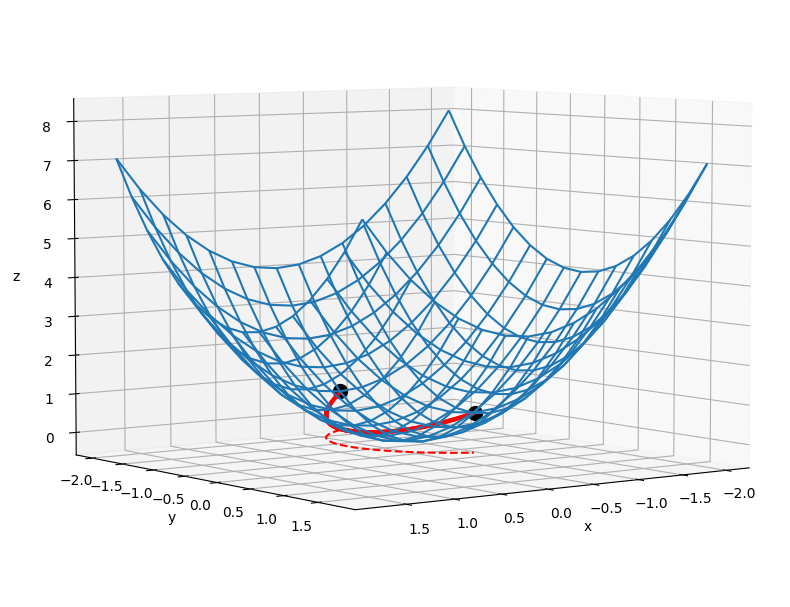
\includegraphics[scale=0.5]{ch13-14.png}
    \end{center}
    Where the red line is the path that starts from the black dot
    $Q = (0, -1, 1)$ and ends on $P = (0, 1, 1)$.
\end{proof}

\end{document}






















